\section{Design}
\label{sec:design}
\fxfatal{Design}

This chapter presents the implemented framework \textit{Banshie} (Benchmark Framework for Information Extraction). The requirements, architecture, design and concrete implementation details are explained and discussed on the following pages.

\subsection{Analysis and requirements}
Provide a platform to benchmark domain-specific information extraction modules.

Designed for Extension and Modularity
OSGi-aware
State of the Art patterns: DI, IoC, Composition over Inheritence, ...
Open Source (Github!)

\url{https://github.com/whiskeysierra/banshie}

\subsection{Architecture}
OSGi, module hierarchy, dependencies

\newpage
\begin{figure}[H]
\centering
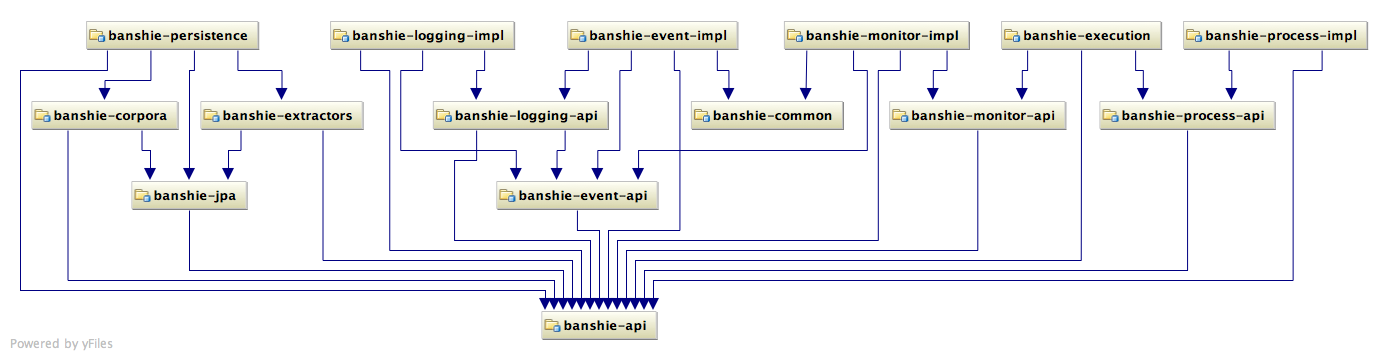
\includegraphics[angle=90, width=0.42\textwidth]{module-dependencies.png}
\caption{Module dependencies}
\label{fig:module-dependencies}
\end{figure}

\newpage
\subsection{Technologies and patterns}

\subsubsection{Dependency Injection}
\gls{DI} is an expression introduced by Martin Fowler in its article \textit{Inversion of Control Containers and the Dependency Injection Pattern} \cite{Fowler:2004}. Dependency Injection specifies the means for obtaining objects in such a way as to maximize reusability, testability and maintainability compared to traditional approaches such as constructors, factories, and service locators \cite{JSR330}. \gls{DI} does this by allowing a class to specify its dependencies and rely on their provision at runtime rather than retrieving them explicitly. This leaves the programmer's code clean, flexible, and relatively free of dependency-related infrastructure \cite{JSR330}.

\paragraph{Guice}
Guice is a lightweight dependency injection framework for Java \cite{Guice}. It's open source and available on \url{https://code.google.com/p/google-guice/}.

The typical code to implement is shown in the following two listings. The first shows a simple \textit{Module}. Modules in Guice are usually used to bind interfaces to concrete classes.

\begin{listing}[H]
\begin{minted}{java}
public final class ProcessModule extends AbstractModule {

    @Override 
    protected void configure() {
        bind(ProcessService.class).to(DefaultProcessService.class);
    }

}
\end{minted}
\caption{Guice module}
\end{listing}

In your classes you usually define a single constructor, annotated with \texttt{@Inject}, and all required dependencies as parameters. The construction of instances and the dependency resolution is done by Guice, no additional boilerplate code is necessary.

\begin{listing}[H]
\begin{minted}{java}
final class DefaultEngine implements Engine {

    private final ProcessService service;

    @Inject
    DefaultEngine(ProcessService service) {
        this.service = service;
    }

}
\end{minted}
\caption{Constructor injection}
\end{listing}

\paragraph{Guice Extensions}
Guice has an extensible plug-in mechanism which allows third parties to provide additional functionality. Banshie uses two official Guice extension extensively: Assisted Inject\footnote{\url{https://code.google.com/p/google-guice/wiki/AssistedInject}} and Multibindings\footnote{\url{https://code.google.com/p/google-guice/wiki/Multibinding}}. Assisted Inject allows the combination of Guice-provided dependencies and user-provided parameters on a single injection point. Multibindings supports the binding and injection of Sets and Maps.

\paragraph{Peaberry}
Guice has no native OSGi support, apart from maybe the OSGi-compatible bundle manifest. To overcome this shortcoming, Peaberry\footnote{\url{https://code.google.com/p/peaberry/}}, a third-party open-source Guice extension offers OSGi-Guice bridge capabilities. It offers \gls{DI} of OSGi dynamic services via Guice's common injection mechanisms and provides a rich an typesafe API to deal with the OSGi service registry and lifecycle events. Figure \ref{lst:peaberry-lifecycle} shows the usage of Peaberry's lifecycle annotations.

\begin{listing}[H]
\begin{minted}{java}
import org.ops4j.peaberry.activation.Start;

public class DefaultCorpusRepository implements CorpusRepository {

    private File basePath = new File("corpora");

    @Start
    public void onStart() {
        basePath.mkdirs();
    }

}
\end{minted}
\caption{Peaberry lifecycle annotation}
\label{lst:peaberry-lifecycle}
\end{listing}

Peaberry even supports the automatic \gls{DI} context creation upon bundle start by using an OSGi extender bundle. Bundles just need to provide the following bundle header to trigger an execution:

\begin{listing}[H]
\texttt{Bundle-Module: org.whiskeysierra.banshie.execution.ExecutionModule}
\caption{Peaberry bundle header}
\end{listing}

Peaberry creates one \texttt{Injector} per bundle, any interaction between bundles is based on standard OSGi services, which allows to combine Peaberry-aware bundles and normal ones.

\subsubsection{Persistence}
Banshie's persistence layer is based on the \gls{JPA} 2.0 Standard. \gls{JPA} allows to build modules without hardcoding for a specific persistence provider or database vendor. Thus allowing to swap implementations later in the development lifecycle without the need to rewrite large portions of the code base. Banshie uses Apache OpenJPA as a \gls{JPA} provider and Apache Derby as the underlying database. Derby is a \gls{RDBMS} written in Java and is distributable as a single Jar file and can be embedded in other applications rather easily.

Using \gls{JPA} in an \gls{OSGi} environment is not a straight forward task. \gls{OSGi} requires bundles to run in different and independent class loaders, while \gls{JPA} heavily relies on classpath scanning and reflection. Both techniques don't work quite well together. Because \gls{JPA}-based persistence is a common requirement, the \citetitle{OSGI:Enterprise} addressed this issue and specifies a standard way to define \textit{Persistence} and \textit{Client bundles} \cite{OSGI:Enterprise}. A persistence bundle is a bundle with the following bundle header:

\begin{listing}[H]
\texttt{Meta-Persistence: META-INF/persistence.xml}
\caption{Persistence bundle header}
\end{listing}

A client bundle is just a bundle that makes use of the \texttt{EntityManagerFactory} provided by the corresponding persistence unit. Most \gls{OSGi} container delegate this part of the \gls{OSGi} specification to third-party libraries and bundles. Apache Aries aims to provide portable implementations in form of standard \gls{OSGi} bundles for those parts of the \gls{OSGi} specification. Banshie uses the JPA module of Apache Aries consisting of \textit{Aries JPA API bundle} and the \textit{Aries JPA container bundle}. To minimize common boilerplate code and manual transaction handling, all \gls{JPA} client bundles use the Guice extension \textit{Guice Persist}. Guice Persist offers AOP-interception for annotated methods as shown in the following listing:

\begin{listing}[H]
\begin{minted}{java}
class DefaultCorpusRepository implements CorpusRepository {

    private EntityManager manager() {
        return provider.get();
    }

    @Transactional
    @Override
    public Corpus get(UUID uuid) {
        return manager().find(CorpusEntity.class, uuid);
    }

}
\end{minted}
\caption{Guice Persist annotation}
\end{listing}

\subsubsection{Build tools}
\paragraph{Maven Bundle Plugin}
With \gls{OSGi} you are forced to provide additional metadata in the JAR's manifest to verify the consistency of your \enquote{class path}. This metadata must be closely aligned with the class files in the bundle and the policies that a company has about versioning. Maintaining this metdata is an error prone chore because many aspects are redundant. bnd's raison d'etre is therefore to remove the chores and use the redundancy to create the manifest from the class files instead of maintaining it by hand. The core task is therefore to analyze the class files and find any dependencies. These dependencies are then merged with instructions supplied by the user \cite{BND}. Since Banshie uses Apache Maven for building its independent modules, the natural choice was to use a Maven Plugin for this, which is provided by the Apache Felix Maven Bundle Plugin \footnote{\url{http://felix.apache.org/site/apache-felix-maven-bundle-plugin-bnd.html}}. The following listing shows the bare minimum of configuration code to use the Maven Bundle Plugin in a POM file.

\begin{listing}[H]
\begin{minted}{xml}
<packaging>bundle</packaging>
...
<build>
    <plugins>
        <plugin>
            <groupId>org.apache.felix</groupId>
            <artifactId>maven-bundle-plugin</artifactId>
        </plugin>
    </plugins>
</build>
\end{minted}
\caption{Maven Bundle Plugin usage}
\end{listing}


\newpage
\subsection{API}

\begin{figure}[H]
\centering
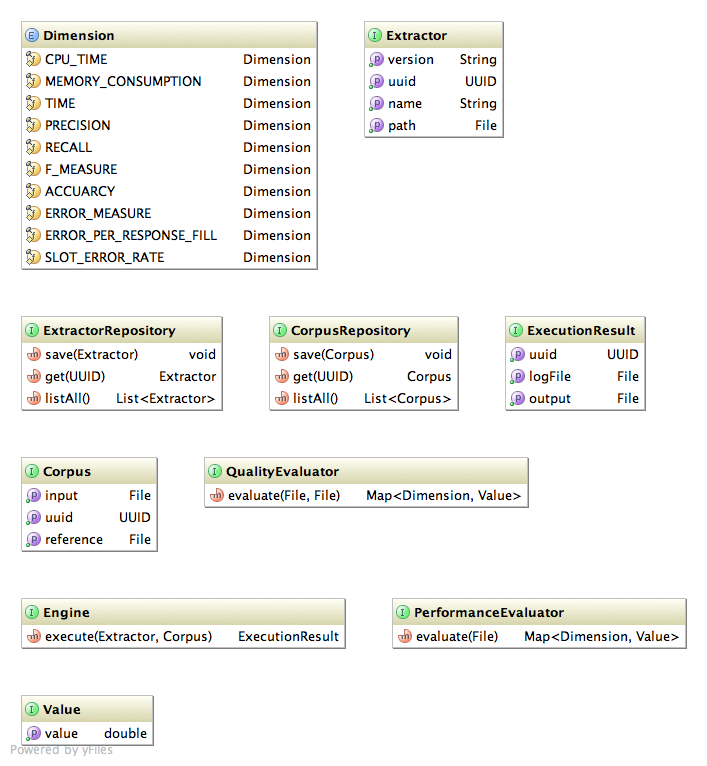
\includegraphics[width=0.9\textwidth]{api.png}
\caption{Banshie API diagram}
\label{fig:api}
\end{figure}

\newpage
Listing \ref{lst:usage} shows the simple basic steps required to perform a single extractor evaluation evaluation.

\begin{listing}[H]
\begin{minted}{java}
// via dependency injection or direct instantiation
final ExtractorRepository extractors = ...;
final CorpusRepository corpora = ...;
final Engine engine = ...;
final PerformanceEvaluator performance = ...;
final QualityEvaluator quality = ...;

final Extractor extractor = extractors.get(extractorId);
final Corpus corpus = corpora.get(corpusId);

final ExecutionResult result = engine.execute(extractor, corpus);
final Map<Dimension, Value> p = 
    performance.evaluate(result.getLogFile());
final Map<Dimension, Value> q = 
    quality.evaluate(corpus.getReference(), result.getOutput());

// handle evaluation results
...
\end{minted}
\caption{Banshie API usage}
\label{lst:usage}
\end{listing}

\subsection{Extractor interface specification}
Since Banshie aims to evaluate the extraction quality as well as the runtime performance of information extraction systems it sets some special requirements for extractors.

Any extractor evaluated by the framework is required to by written in Java and compiled for Java 1.6 or higher as a single executable Jar file. Being packaged as a single file requires the extractor to bundle every external dependency into a single archive. Embedding third-party java libraries can be accomplished by utilizing the \textit{JarJar}\footnote{\url{https://code.google.com/p/jarjar/}} tool. External files like models and training data can packaged as standard classpath resources.

For a Jar file to be executable it has to have a manifest file, i.e. META-INF/MANIFEST.MF), and a manifest header as shown in the following listing:

\begin{listing}[H]
\texttt{Main-Class: org.whiskeysierra.banshie.example.opennlp.Main}
\caption{Extractor manifest header}
\end{listing}

The extractor can than be started using the following command.

\begin{listing}[H]
\texttt{java -jar extractor.jar}
\caption{Extractor java execution command}
\end{listing}

Since an extractor under evaluation has a single input, the test document, and a single output, the annotated hypothesis, the natural choice was to utilize standard streams, standard input (\textit{stdin}) and and standard output (\textit{stdout}) respectively. The test document is passed to the extractor in UTF-8 encoding. Whether the extractor streams the document or reads it into memory as a whole is up the extractor. The output format is \gls{XML} as defined by the schema shown in listing \ref{lst:xml-schema}.

\begin{listing}[H]
\inputminted{xml}{../../../../../banshie-api/src/main/resources/schema.xsd}
\caption{Banshie XML Schema}
\label{lst:xml-schema}
\end{listing}

As shown in listing \ref{lst:xml-example}, the defined output format is a very simple XML document containing the original document and all found spans annotated with the corresponding type as a simple XML element tag.

\begin{listing}[H]
\inputminted{xml}{../../../../../banshie-api/src/main/resources/example.xml}
\caption{Banshie XML Example}
\label{lst:xml-example}
\end{listing}

The span element has three attributes: \texttt{type}, \texttt{start} and \texttt{end}. Type is one of \texttt{person}, \texttt{organiazation} or \texttt{location}, based on the ENAMEX tags developed for the Message Understanding Conference \cite{Grishman:1996}.

The attribtues \texttt{start} and \texttt{end} define the character offset of the span in the original document to support character based association of spans in the reference and the predication.

\subsection{Reference-hypothesis association}
Evaliex \cite{Linsmayr:2010} uses the \enquote{General Greedy Mapping Algorithm} as proposed by \citeauthor{Douthat:1998} in 1998 \cite{Douthat:1998}. 

